\section{Observability}
    OpenTelemetry refers to observability as \cite{otel-o}:
    \begin{quote}
 ``The ability to understand the internal state by examining its output. In the context of a distributed system, being able to understand the internal state of the system by examining its telemetry data.''
    \end{quote}
    In the case of the Erlang programming language, we describe respectively two different ways to observe a running Erlang system: erlang:trace and OpenTelemetry.
    
    \subsection{erlang:trace}
        The Erlang programming language gives the users different ways to observe the behaviour of a system, one of those is the interface \texttt{erlang:trace}. According to the documentation: ``The Erlang run-time system exposes several trace points that can be observed, observing the trace points allows users to be notified when they are triggered'' \cite{erl-t}. One can observe function calls, messages being sent and received, process being spawned, garbage collecting and more. 
        \begin{figure}[!ht]
        \centering
        \begin{minted}{erlang}
            -spec trace(PidPortSpec, How, FlagList) -> integer()
               when
                   PidPortSpec ::
                       pid() |
                       port() |
                       all | processes | ports | existing | existing_processes | existing_ports | new |
                       new_processes | new_ports,
                   How :: boolean(),
                   FlagList :: [trace_flag()].
        \end{minted}
        \caption{erlang:trace/3 specification.}
\end{figure}

    Nevertheless, in Erlang trace there is no default way to follow a message and get its whole execution trace. This is a missing feature that is crucial for observing a program functioning and being able to connect an application to our oscilloscope.  This is where the OpenTelemetry framework comes in.

\subsection{OpenTelemetry}
    According to OpenTelemetry website \cite{otel-o}: OpenTelemetry is an open-source, vendor-agnostic observability framework and toolkit designed to generate, export and collect telemetry data, in particular traces, metrics and logs. OpenTelemetry provides a standard protocol, a single set of API and conventions and lets the user own the generated data, allowing to switch between observability backends freely.
   
   OpenTelemetry is available for a plethora of languages \cite{otel-l}, including Erlang, although, as of writing this, only traces are available in Erlang \cite{otel-in}.
     
    The Erlang Ecosystem Foundation has a working group focused on evolving the tools related to observability, including OpenTelemetry and the runtime observability monitoring tools \cite{obs-group}. 
    
    \subsubsection{Traces}
        Traces are why we are basing our program on top of OpenTelemetry, traces follow the whole path of a request in an application, and they are comprised of one or more spans \cite{otel-t}. Traces can propagate to multiple services and record multiple paths in different microservices \cite{otel-dt}. 
        
        \paragraph{Span} A span is a unit of work or operation. Multiple spans can be assembled into a trace and can be causally linked (\cref{fig:monitor}). The spans can have a hierarchy, where \textit{root spans} represent a request from start to finish and a child span the requests that are completed inside the root span \cite{otel-dt}. We will see in later sections how this can relate to what the oscilloscope does.

    The notion of spans and traces allows us to follow the execution of a request and carry a context. Spans can be linked to mark causal relationships between multiple spans \cite{otel-t}. This relation can be represented in the oscilloscope via \textbf{probes}, we will present how spans relate to probes in following sections.
    \begin{figure}[H]
    \begin{minted}{json} 
{
  "name": "oscilloscope-span",
  "context": {
    "trace_id": "5b8aa5a2d2c872e8321cf37308d69df2",
    "span_id": "5fb397be34d26b51"
  },
  "parent_id": "051581bf3cb55c13",
  "start_time": "2022-04-29T18:52:58.114304Z",
  "end_time": "2022-04-29T22:52:58.114561Z",
  "attributes": {
    "http.route": "some_route"
  },
}
    \end{minted}
    \caption{Example of span from the OpenTelemetry website \cite{otel-t}. The span has a parent, indicating that child and parent spans are related and are both part of the same trace.}%
    \end{figure}

    \subsubsection{Monitoring OpenTelemetry spans}
        In OpenTelemetry, the user can export their traces export to backends and monitoring such as Jaeger (\cref{fig:monitor}), Zipkin, Datadog \cite{otel-exp}. There, a user can analyse the traces to troubleshoot their programs by observing the flow of the requests \cite{jg}. These monitoring tools give extensive details about a running system, but may fail to capture essential timeliness requirements and performances issues early enough.
        
        Our oscilloscope is a kind of monitoring tool, one that gives precise statistical insights about a running system. It is clear that the oscilloscope does not have the same capabilities as Datadog \cite{datadog} might have, where you can observe cloud instances, instances cost, dependency graphs. But the oscilloscope can nevertheless provide precise insights about dependency, overload thanks to the $\Delta$QSD paradigm. 

        This is also the reason why the adapter includes OpenTelemetry macros. The oscilloscope can be put next to a monitoring tool where one might export spans to, so that an engineer might consult the monitoring tool to get the global picture of a running app, as the oscilloscope can provide more precise insights to understand the system's behaviour. 
       \begin{figure}[H]
            \centering
            \begin{subfigure}{.5\textwidth}
                \centering
                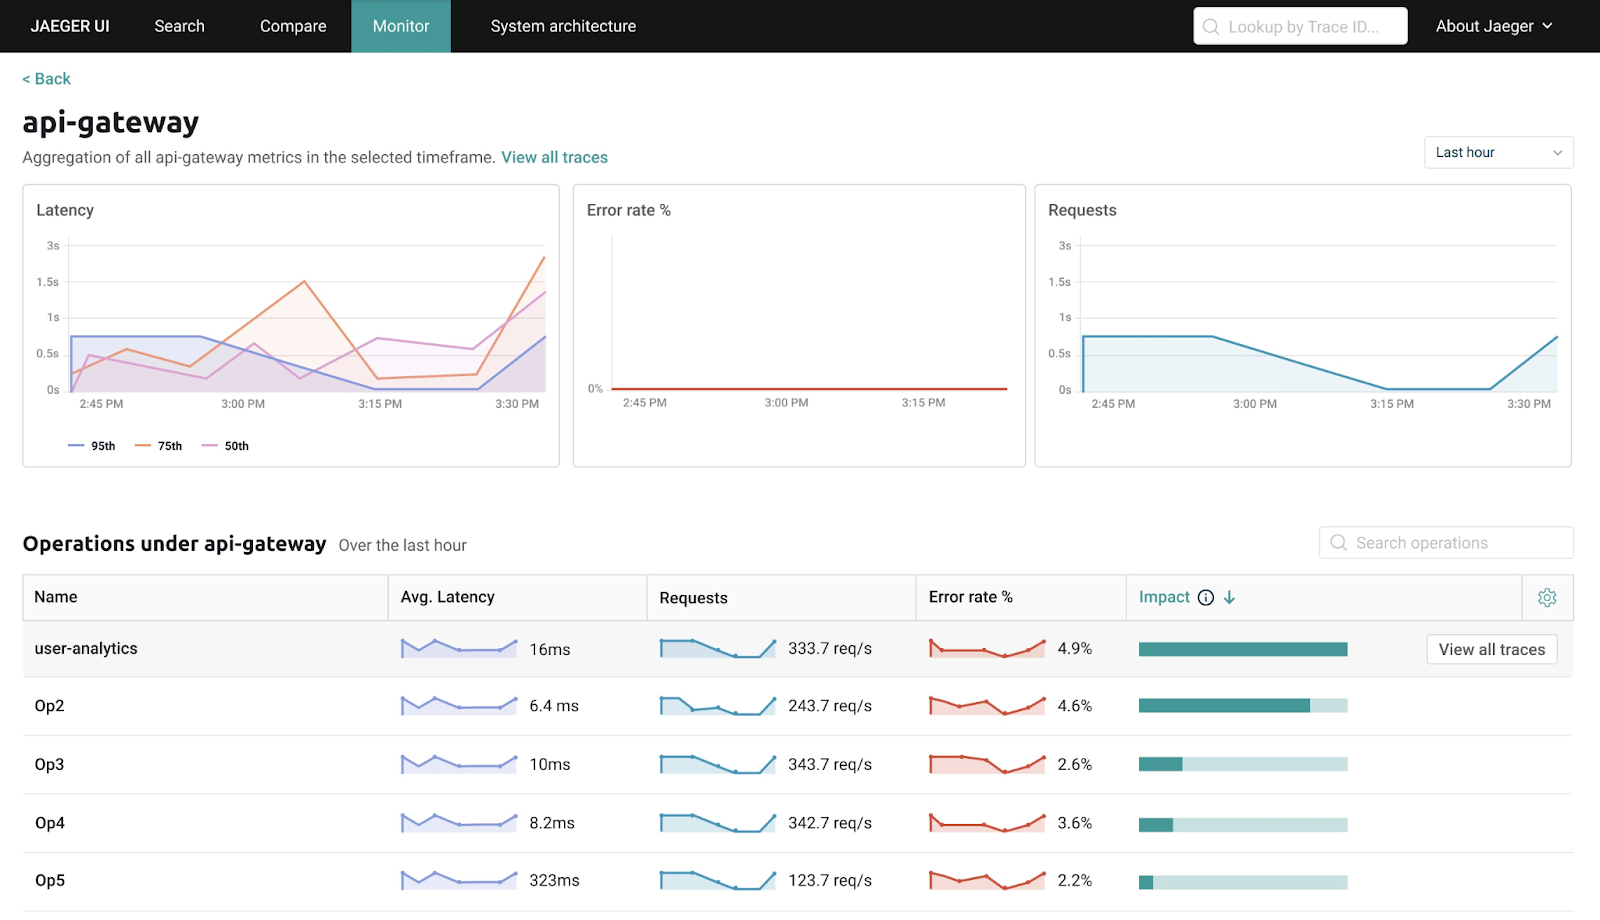
\includegraphics[width=0.98\textwidth]{img/jaeger.png}
                \label{fig:jag}
            \end{subfigure}%
            \begin{subfigure}{.5\textwidth}
                \centering
                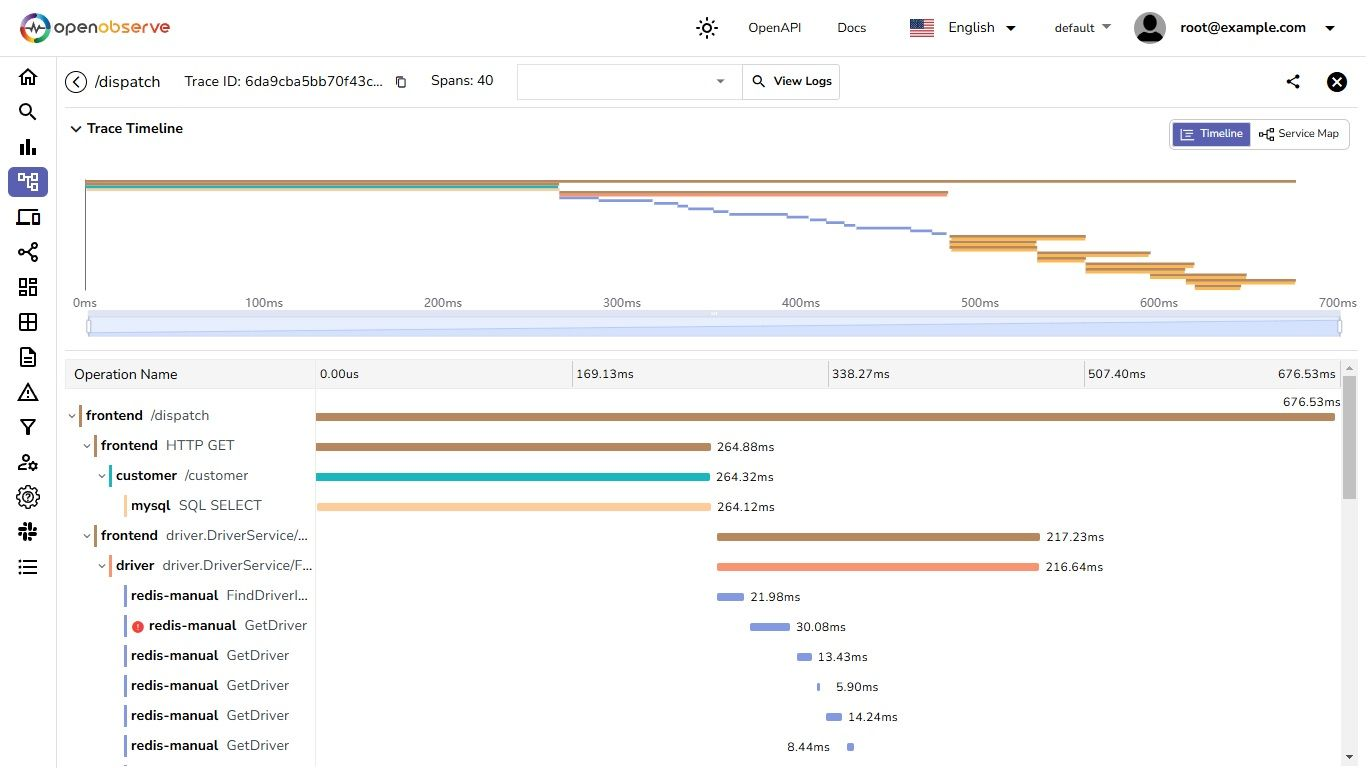
\includegraphics[width =0.98\textwidth]{img/jaeger2.jpg}
                \label{fig:openobs}
            \end{subfigure}
            \caption{\textbf{Left}: Jaeger interface \cite{otel-p}. \textbf{Right}: Analysis of a span on OpenObserve. \cite{tr-e}}
            \label{fig:monitor}
            \end{figure}

    \subsubsection{Span macros}
        OpenTelemetry provides macros to start, end and interact with spans in Erlang, the following code excerpts are taken from the OpenTelemetry instrumentation wiki. \cite{otel-in}
        \paragraph{?with\_span}
            \texttt{?with\_span} creates active spans. An active span is the span that is currently set in the execution context and is considered the ``current'' span for the ongoing operation or thread. \cite{active-s}
        \begin{minted}{erlang}
parent_function() ->
    ?with_span(parent, #{}, fun child_function/0).
child_function() ->
%% this is the same process, the span parent set as the active
%% span in the with_span call above will be the active span in this function
    ?with_span(child, #{},
               fun() ->
     %% when this function returns, child will complete.
               end).
        \end{minted}
        \paragraph{?start\_span}
            \texttt{?start\_span} creates a span which isn't connected to a particular process, it does not set the span as the current active span.
        \begin{minted}{erlang}
SpanCtx = ?start_span(child),
Ctx = otel_ctx:get_current(),
proc_lib:spawn_link(fun() ->
                        otel_ctx:attach(Ctx),
                        ?set_current_span(SpanCtx),
                        ?end_span(SpanCtx)
                    end),
        \end{minted}
        \paragraph{?end\_span}
            \texttt{?end\_span} ends a span started with \texttt{?start\_span}

